\documentclass[11pt]{report}
\usepackage[utf8]{inputenc}
\usepackage[danish]{babel}
\usepackage [T1]{fontenc}
\usepackage[margin=2.5cm]{geometry}
\usepackage[hidelinks]{hyperref}
\usepackage{graphicx}
\graphicspath{{figures/}{Billeder/}}
\usepackage{listings}
\usepackage{color}
\usepackage{adjustbox}
\usepackage{tocloft}

\definecolor{bluekeywords}{rgb}{0.13,0.13,1}
\definecolor{greencomments}{rgb}{0,0.5,0}
\definecolor{turqusnumbers}{rgb}{0.17,0.57,0.69}
\definecolor{redstrings}{rgb}{0.5,0,0}

\lstdefinelanguage{FSharp}
                {morekeywords={let, new, match, with, rec, open, module, namespace, type, of, member, and, for, in, do, begin, end, fun, function, try, mutable, if, then, else},
    keywordstyle=\color{bluekeywords},
    sensitive=false,
    morecomment=[l][\color{greencomments}]{///},
    morecomment=[l][\color{greencomments}]{//},
    morecomment=[s][\color{greencomments}]{{(*}{*)}},
    morestring=[b]",
    stringstyle=\color{redstrings}
    }
\usepackage{amsmath}
\title{Cupcake}
\author{
    Asger Hermind Sørensen\\
    cph-as466@cphbusiness.dk\\
    asgerhs\\
    A klassen\\
  &
    William Sehested Huusfeldt\\
    cph-wh106@cphbusiness.dk\\
    WSHuusfeldt\\
    A klassen
  \and
    Andreas Vikke\\
    cph-av105@cphbusiness.dk\\
    AndreasVikke\\
    A klassen\\
  &
    Martin Eli Frederiksen\\
    cph-mf237@cphbusiness.dk\\
    Krigermus\\
    A klassen
}

\date{\today}

\begin{document}
\maketitle

\renewcommand{\cftchapleader}{\cftdotfill{\cftdotsep}}
\tableofcontents
\newpage

\chapter*{1. Indledning}
\addcontentsline{toc}{chapter}{1. Indledning}
Projektet omhandler en webapplikation, hvor kunden er en forretning
der sælger cupcake. Formålet var at udvikle en hjemmeside, produktet, med en tilhørende database, hvor kunder kan registrere sig som brugere, se og bestille varer samt administrere tidligere bestillinger. Ydermere er der udviklet et værktøj til ejeren af forretningen, som giver mulighed for at administrere brugere og deres bestillinger.
\newpage

\chapter*{2. Baggrund}
\addcontentsline{toc}{chapter}{2. Baggrund}
\section*{2.1. Virksomheden}
\addcontentsline{toc}{section}{2.1. Virksomheden}
\textit{‘C for CupCake’} er en lille familievirksomhed som har
beliggenhed på Nørregade 2. De har lavet cupcakes i et lille år, og vil derfor gerne
have en hjemmeside i håbet om at øge salget i deres virksomhed. De har
derfor taget kontakt til os med deres ide, hvorefter vi har udviklet
systemet til dem.

\section*{2.2. Virksomhedens krav}
\addcontentsline{toc}{section}{2.2. Virksomhedens krav}
\begin{itemize}
  \item Hjemmesiden skal kunne give en kunde mulighed for at købe en
    cupcake, hvor de selv vælger hvad for en top og bund de vil have,
    ud fra de muligheder som virksomheden producere. 
  \item Kunden skal kunne have oversigt over sine ordre. 
  \item Kunden skal oprette sig som kunde inde på siden, og kan kun få
    adgang til at købe produkter hvis de har en konto.
  \item Kunde skal kunne tilføje penge til deres konto, som de bruger
    til at betale for de cupcakes som de bestiller.
  \item Kunden skal kunne se ud fra deres ordre hvornår den er klar
    til at blive hentet i butikken.
\end{itemize}


\section*{2.3. Virksomhedens vision}
\addcontentsline{toc}{section}{2.3. Virksomhedens vision}
Det som virksomheden gerne vil opnå med hjemmesiden er at øge deres salg. Derudover vil de gerne kunne lave reklamer til deres hjemmeside, således at potentielle kunder kan se deres produkter og købe dem uden at tage ned i butikken.
\newpage

\chapter*{3. Sprog og programmer}
\addcontentsline{toc}{chapter}{3. Sprog og programmer}
\textbf{Loaklt:}
\begin{itemize}
  \item Windows - Linux - MacOS.
  \item Java v. 8.
  \item Mysql v. 8.0.14.
  \item MySQL Workbench v. 8.0.15.
  \item Github / Github Desktop.
  \item Netbeans v. 8.2.
  \item Maven v. 3.5.2.
\end{itemize}
\textbf{Server:}
\begin{itemize}
  \item Linux - Ubuntu 18.10.
  \item Java Openjdk 11.
  \item Mysql v. 8.0.14.
  \item Maven v. 3.5.2.
\end{itemize}
\newpage

\chapter*{4. ER Diagram}
\addcontentsline{toc}{chapter}{4. Baggrund}
Databasen består af 5 tabeller, Users, Orders, OrderLines, Invoices og CupcakeParts.
\begin{enumerate}
  \item Users tabellen har et username som PRIMARY key og email som
    UNIQE index da ingen af disse må være ens i tabellen.
  \item Orders har et orderId som PRIMARY key, dette id har også AUTO
    INCREMENT for nemt at tælle id’et op.
  \item OrderLines har orderId, CupcakeTopId og CupcakeBottomId som PRIMARY keys.
  \item Invoices har invoiceId som PRIMARY ket, dette id har også AUTO
    INCREMENT for nemt at tælle id’et op.
  \item CupcakeParts har id som PRIMARY KEY, dette id har også AUTO
    INCREMENT for nemt at tælle id’et op. Specielt ved denne tabel er
    at partType er en ENUM med værdierne “TOP” og “BOTTOM”.
\end{enumerate}
\begin{center}
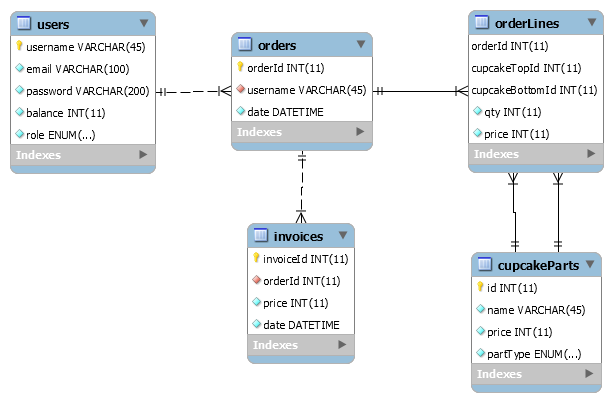
\includegraphics[width=15cm]{Er.png}
\end{center}
\newpage

\chapter*{5. Navigationsdiagram}
\addcontentsline{toc}{chapter}{5. Navigationsdiagram}
\textbf{Customer Navigations diagram:}\\
Brugeren/kunden kan se sine ordre fra sin brugerside, customer.jsp. I
venstre halvdel af siden kan brugeren klikke på enten “account
information” eller “orders”, ved at klikke på “orders” bliver brugeren
navigeret til en side (customerorderlist.jsp) hvor der på højre
halvdel kommer en liste frem. Denne liste bliver hentet fra
databasen. For hver linje (ordre) kan brugeren se detaljer ved at
klikke på “Show order”. Brugeren bliver dirigeret til order.jsp, hvor
hele ordrens indhold bliver vist, dette værende Cupcake top, bund,
mængde og pris. Det er på denne side muligt at komme tilbage til den
foregående side ved at trykke på “Back”. \\\\
\begin{center}
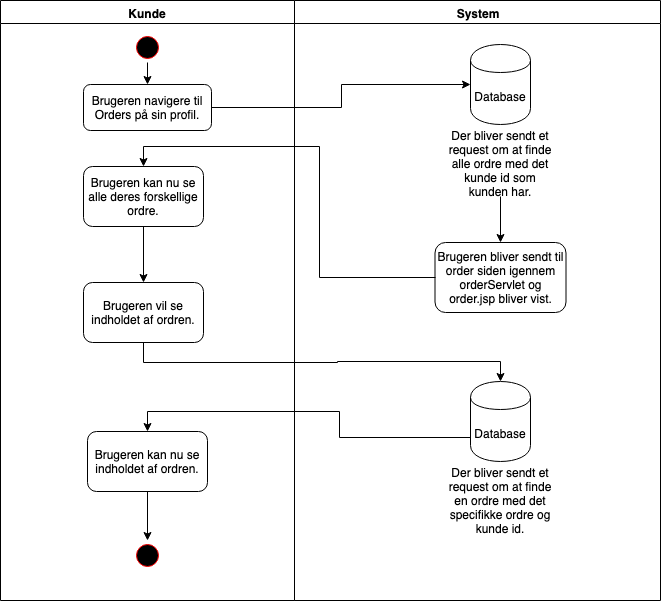
\includegraphics[width=14cm]{OrdersCupCake.png}
\end{center}
\newpage

\noindent
\textbf{Admin navigations diagram:}\\
For en admin der gerne vil se alle brugerne, har admin mulighed for det på admin.jsp, hvor alle brugeres brugernavn og ID er vist. Først får admin en liste over alle kunder i systemet; navn, email og en knap der går videre til kundes ordre. Herfra kan admin vælge at vise alle ordrene i systemet eller vise alle ordrene for en specifik kunde. Ordene vil vises som en liste med kunde navn, id, dato og en knap til at vise detaljer på ordren. Detalje vinduet vil vise de linjer der er købt og prisen på linjerne samt total prisen. Den sidste mulighed som admin har er at skifte kodeord som foregår gennem navigations diagrammet til at skifte kodeord.\\\\
\begin{center}
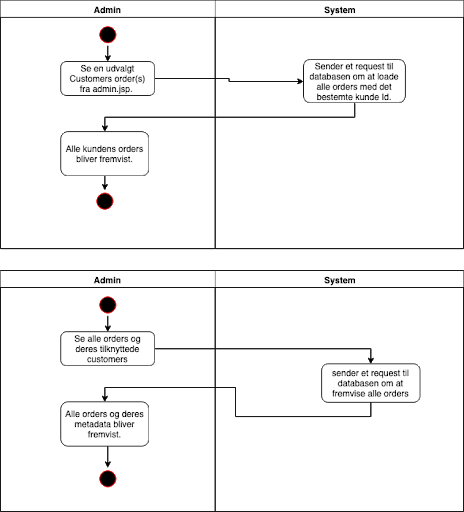
\includegraphics[width=15cm]{Admin.png}
\end{center}
\newpage

\noindent
\textbf{Navigationsdiagram over at skifte kode:}\\
Ved customer.jsp (også muligt for admin, her admin.jsp) er det muligt, udover at se ordre, at skifte kodeord. Dette gøres ved at trykke på “Account information”, hvor changepassword.jsp bliver inkluderet i customer.jsp siden. Her vil tre tekst bokse komme frem hvor brugeren bliver spurgt om at indtaste sit nuværende kodeord og et nyt kodeord to gange. Disse bliver brugt som parametre, som har betydning for, om brugeren får en fejlbesked eller om kodeordet bliver skiftet. Command-klassen der bliver benyttet validerer brugeren ved at hente brugernavnet fra den kørende session og tjekker om brugeren har skrevet det rigtige nuværende kodeord. Stemmer de ikke overens bliver brugeren forwarded til error.jsp, som bliver fanget af ajax() metoden, som fremviser en error header med den error message der er defineret. Bliver brugeren valideret tjekker execute metoden i command-klassen om felterne er fyldt, dernæst om det nye kodeord (skrevet to gange) matcher hinanden. Er dette tilfældet bliver kodeordet ændret og gemt i databasen. Er det ikke tilfældet at kriterierne er opfyldt bliver brugeren forwarded til error.jsp, som bliver fanget af ajax() metoden igen, som fremviser en error header hvor der står - brugeren skal skrive kodeordene på ny.\\\\
\begin{center}
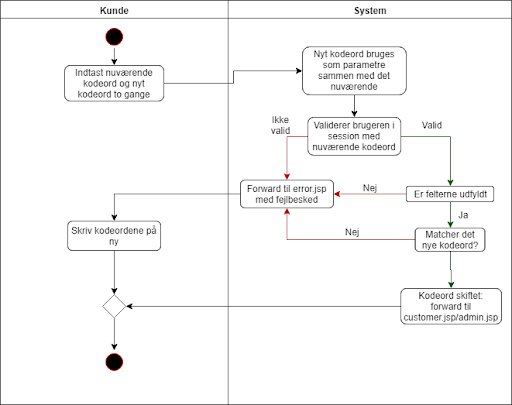
\includegraphics[width=15cm]{ChangePasswordCupCake.png}
\end{center}
\newpage

\noindent
\textbf{Login navigations diagram:}\\
Når en bruger først ankommer til forsiden af hjemmesiden, kommer de hen til login.jsp. Hvis en bruger ikke er logget ind og trykket på “Cupcake” logoet bliver de også videresendt til login.jsp. Her bliver en bruger bedt om at indtaste brugernavn og adgangskode, hvor de så til sidst kan trykke på login. Brugernavn og kodeord bliver sendt som parametre, og checket i databasen om parametrene er korrekte. Hvis en af de to parametre ikke stemmer overens med dataen i databasen, bliver det videresendt til error.jsp som bliver fanget af ajax() metoden, som fremviser den header der er blevet sat. Stemmer både brugernavn og password overens med dataen i databasen, bliver der til sidst checket om brugeren er en admin bruger eller en almindelig bruger. Hvis brugeren er admin bliver brugeren videresendt til admin,jsp, hvis ikke bliver brugeren sendt til customer.jsp.\\\\
\begin{center}
\includegraphics[width=15cm]{LoginCupCake.png}
\end{center}
\newpage

\noindent
\textbf{Navigationsdiagram over register:}\\
\textbf{\textit{Skal en bruger oprette sig som kunde}}, skal de igennem
register.jsp. Herinde har de tre felter hvor de skal indtaste e-mail,
brugernavn og kodeord, og dette er parametrene som bliver sendt til
registerCommand.java. registerCommand checker først om e-mail feltet,
brugernavn feltet og kodeord feltet om nogle af disse er tomme. Hvis
nogle af dem er tomme bliver de videresendt til error.jsp, som bliver
fanget af vores ajax() metode, som fremviser den error header som der
er sat. Hvis felterne ikke er tomme bliver der derefter checket
hvorvidt der allerede er en eksisterende bruger med den indtastede
e-mail eller brugernavn. Hvis der allerede er en eksisterende bruger,
får brugeren endnu en error header fra ajax() som fremviser den error
header der er blevet sat. Hvis felterne ikke er tomme, og der ikke er en eksisterende bruger så bliver brugeren oprettet i databasen og videresendt til login.jsp.\\\\ 
\begin{center}
\includegraphics[width=15cm]{RegisterCupCake.png}
\end{center}
\newpage

\noindent
\textbf{Navigationsdiagram over cart}\\
\textbf{\textit{Skal en bruger have flere penge på sin konto}}, så skal
brugeren navigere sig til cart.jsp. Et sted på siden (per tids
skrivning, nederst til venstre), vil brugeren kunne se et felt hvor de
kan sætte penge ind på deres konto. Når brugeren har indtastet et
beløb (max 25 tegn) og får trykket add balance, bliver brugeren hentet
igennem sessionen og beløbet bliver gemt som parameter og sendt til
databasen. Databasen tager imod ændringerne og opdatere brugerens
beløb. Til sidst videresendes brugeren tilbage til cart.jsp.\\
\textbf{\textit{Har en bruger fortrudt et salg eller er kommet til at slå den
  forkerte vare ind}}, så kan brugeren, igen inde i cart.jsp, fjerne
bestillingen. Brugeren vælger til venstre for fjern knappen, som
findes på hver linje, hvor mange af den linje man vil fjerne fra sin
cart. Når brugeren derefter har trykket på slet, sendes top id'et og
bund id'et som parametre igennem command controlleren. I
deleteLineItemCommand.java sikres der at linjen ikke er null/tom, og
opdatere derefter mængden på linjen. Ellers så bliver der sendt en
error besked til brugeren.\\
\textbf{\textit{Når brugeren en færdig og gerne vil købe}}, trykker brugeren på
“checkout”. Sessionen checker derefter om ordrens pris er højere end
den balance som brugeren har, er den det bliver brugeren videresendt
til error.jsp og får ligeledes af vide at deres balance er for lav i
forhold til købet. Er balancen lig med eller højere end købs totalen
bliver balancen opdateret i databasen for brugeren og ordren bliver
oprettet for brugeren. Til sidst bliver brugeren videresendt til
cart.jsp.\\\\
\begin{center}
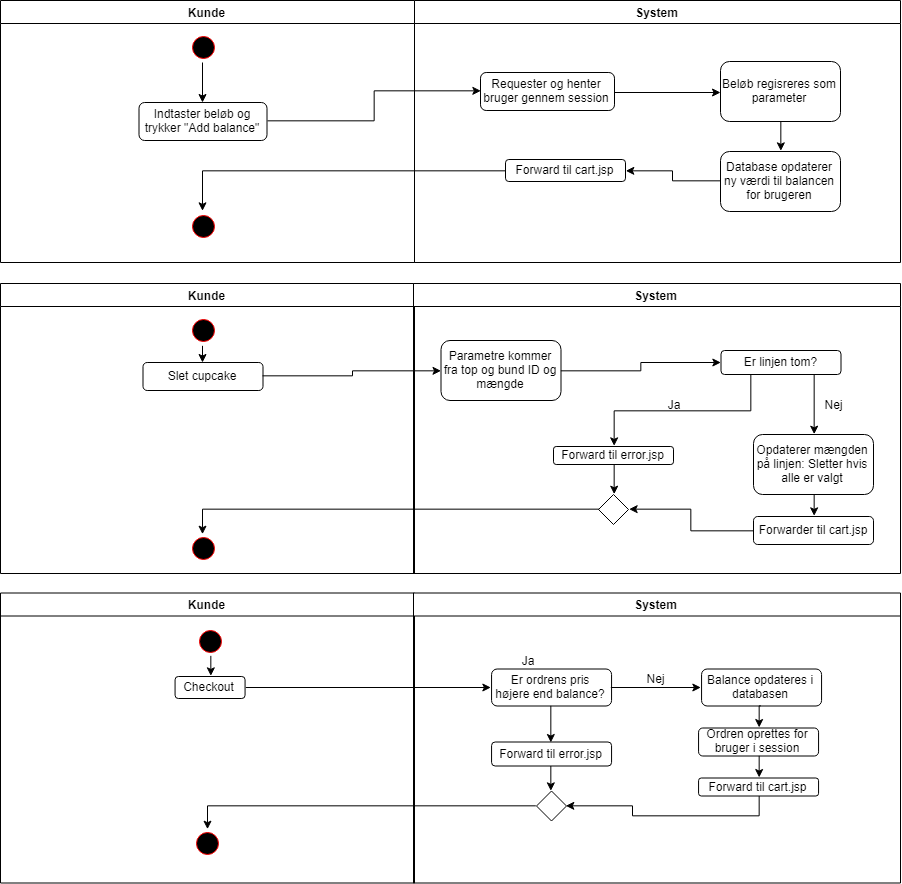
\includegraphics[width=13cm]{CartCupcake.png}
\end{center}
\newpage

\noindent
\textbf{Navigationsdiagram over shop}\\
Inde på shop.jsp kan brugeren vælge imellem nogle forskellige toppe og bunde til sin cupcake. Kunden har valgt hvilken top og bund de vil have, samt hvor mange af dem de vil have, cupcakenes id og mængden af dem bliver brugt som parametre, og til sidst har kunden trykket tilføj til kurv. Her efter bliver den valgte top og bunds id gemt sendt videre igennem productCommand.java  som parametre i sessionen for shoppingcart.\\\\
\begin{center}
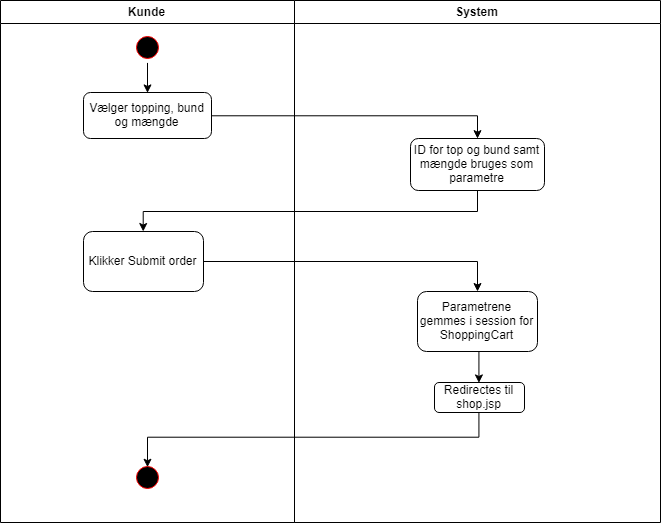
\includegraphics[width=15cm]{ShopCupcake.png}
\end{center}
\newpage

\noindent
\textbf{Navigations diagram over header oversigten}\\
Som tilføjelse til hver side på serveren er der tilføjet en header,
der fungerer som en navigationsbar. Det er både almindelige brugere og
admin brugere som kan benytte sig af denne, og det fungerer som den
primære metode at navigere rundt på serveren. Headeren vil være forskellig alt efter, om brugeren er logget ind eller ej. Som udgangspunkt er brugeren ikke logget ind og kan benytte sig af “Login” tasten, som her forwarder til login.jsp, hvor login processen forekommer. Det er også muligt at registrere sig som bruger ved at bruge “Register” tasten.
Det er ikke muligt at tilgå shop.jsp, cart.jsp eller
customer.jsp/admin.jsp uden at være logget ind. Shop og basket bliver
tilgængelig ved login samt customer.jsp/admin.jsp, der fungerer som
standard siden efter login.\\\\
\begin{center}
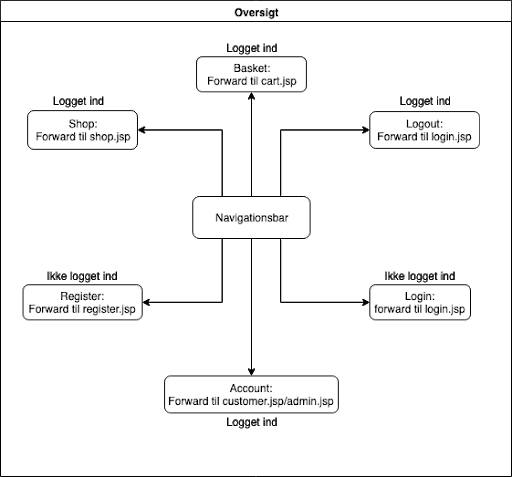
\includegraphics[width=15cm]{HeaderCupCake.png}
\end{center}

\chapter*{6. Sekvens diagrammer}
\addcontentsline{toc}{chapter}{6. Sekvens diagrammer}
\textit{Sekvensdiagram for en bruger der har valgt en cupcake og nu gerne vil købe den:}
\begin{center}
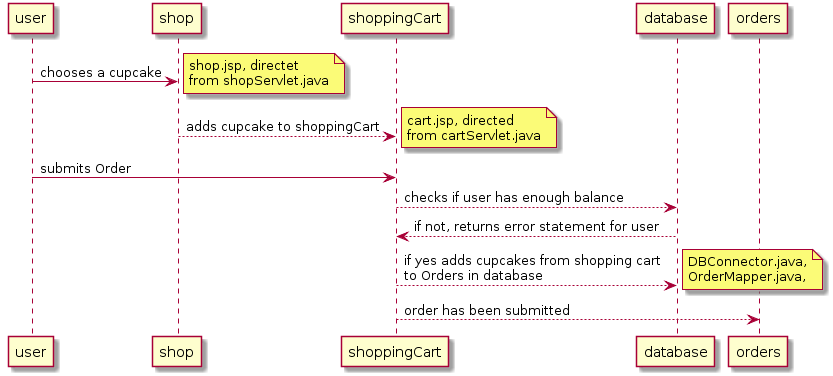
\includegraphics[width=15cm]{SekvensDiagramCupCake.png}
\end{center}
Når en bruger gerne vil købe en cupcake, skal de igennem til shop siden der er på shop.jsp. Herinde vælger de så den cupcake de gerne vil have. Når den er valgt og de trykker submit, så bliver den tilføjet til shopping carten, men brugeren forbliver på shop siden. Når brugeren dernæst er færdig med at vælge de cupcakes de skal have, kan de dirigere sig selv til shopping cart siden (shoppingCart.jsp), hvor brugeren kan kigge på alle deres valgte cupcakes. Brugeren bekræfter med sig selv at de ikke skal have mere, og submitter ordren fra shopping carten. Her checker databasen efter om brugerens balance er høj nok i forhold til det som brugeren gerne vil købe. Hvis balancen er lavere end total prisen, bliver der retuneret et error statement fra error.jsp, som bliver fanget af ajax(), som fremviser en error header. Når balancen er høj nok kan brugeren afslutte deres køb, og ordren bliver gemt under orders på databasen, som også bliver fremvist på order.jsp.

\chapter*{7. Struktur}
\addcontentsline{toc}{chapter}{7. Struktur}
Der er blevet brugt en tre lags arkitektur som struktur. Serveren
består overordnet af et data, præsentation og logik lag. Både data og
logik laget er blevet udvidet for lettere orientering. Data laget er
blevet delt op i tre mapper, første mappe bestående af klasser, der
forbinder severen til databasen. Dernæst en mappe der består af
mapper-klasserne og til sidst en mappe bestående af interfaces til
mapper-klasserne. Logik laget er som data laget også delt op, her i
fire dele. En mappe hvor serverens controller-klasser ligger, en mappe
for command-klasserne og en for model-klasserne og til sidst en mappe
for enum model-klasser. Sidst er der præsentations laget hvor alle servlets ligger.
\begin{center}
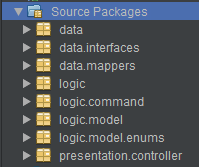
\includegraphics[width=5cm]{Arkitektur.png}
\end{center}
Serveren består ydermere af .jsp klasser, som bestemmer hvordan siderne på sitet vises og hvilke command-klasser der skal bruges.
Det blev valgt, at udvalgte .jsp klasser skulle være skjulte og dermed
kun gøre det muligt at tilgå disse sider hvis man bliver videresendt
fra en servlet. I data laget ligger de klasser, som “snakker” med
databasen. Der er tre klasser der sørger for at oprette forbindelse
til databasen, som er grundlaget der bliver brugt til
mapper-klasserne, som består af metoder med SQL Query kode. Udover
mapper-klasserne er der tilhørende interfaces, som sikrer at
mapper-klasserne har de rigtige metoder. Dernæst er der
controller-klasserne der fungerer som mellemled mellem
præsentationslaget og datalaget. Dette styrker sikkerheden gennem
serveren, så brugeren ikke direkte tilgår databasen ved at navigere
rundt på siden og gøre brug af dets funktioner. Command-klasserne
består af al den data der skal bruges for at udføre en bestemt
handling. Dette f.eks. Værende at skifte kodeord for brugeren. Sidst er der servletterne, der forwarder og redirecter brugeren til de rigtige sider. Nogle af servletterne tjekker f.eks. Om man er logget ind før de videresender en til den side man er igang med at tilgå.

\chapter*{8. Særlige forhold}
\addcontentsline{toc}{chapter}{8. Særlige forhold}
Ved validering af brugeren gøres dette ved at tjekke, om det indtastede brugernavn og kodeord stemmer overens med en bruger registreret i databasen. Dermed bliver det tjekket ved brug af en SQL-query. Ved denne validering er der gjort forsøg på sikkerhed i form af, at kodeordet bliver krypteret. Krypteringen blev gjort muligt af java-klassen MessageDigest samt DatatypeConverter.
Eksempelvis i funktionen der giver brugeren mulighed for at skifte
kodeord, er det aktuelt med både at validere brugeren og at kryptere
det nye kodeord. En tilføjelse der krævede alternative løsninger var sortering af ordre
på customerorderlist.jsp og orderlist.jsp siden hvor der blev brugt
JavaScript.\\

\begingroup
\renewcommand{\cleardoublepage}{}
\renewcommand{\clearpage}{}
\chapter*{9. Manglende implementer}
\addcontentsline{toc}{chapter}{9. Manglende implementer}
\endgroup
\noindent
Der mangler at blive implementeret tests til serveren. Der er per tids skrivning ingen test til serveren. 
Ydermere er der ikke blev opsat en gennemarbejdet backup af
databasen. Som en hurtig løsning er der blevet lavet en manuel backup,
men kun en enkelt. Dette er vel at mærke ikke en vedvarende løsning,
den forældes hurtig ved f.eks. At nye brugere registrerer sig på
serveren. Derfor vil en automatisk backup af databasen være ideel. Det
vil betyde at backup-dataen er opdateret og at risikoen for mistet
data mindskes.\\

\begingroup
\renewcommand{\cleardoublepage}{}
\renewcommand{\clearpage}{}
\chapter*{10. Links og referencer}
\addcontentsline{toc}{chapter}{10. Links og referencer}
\endgroup
\begin{itemize}
  \item CupCake Webshop: \url{http://andreasvikke.dk/CupCake/}
  \item GitHub: \url{https://github.com/Krigermus/CupCake/}
  \item JavaDoc: \url{http://andreasvikke.dk/CupCake-javadoc/}
\end{itemize}

 \newpage

\end{document}

